\documentclass[12pt]{article}\usepackage[]{graphicx}\usepackage[]{color}
%% maxwidth is the original width if it is less than linewidth
%% otherwise use linewidth (to make sure the graphics do not exceed the margin)
\makeatletter
\def\maxwidth{ %
  \ifdim\Gin@nat@width>\linewidth
    \linewidth
  \else
    \Gin@nat@width
  \fi
}
\makeatother

\definecolor{fgcolor}{rgb}{0.345, 0.345, 0.345}
\newcommand{\hlnum}[1]{\textcolor[rgb]{0.686,0.059,0.569}{#1}}%
\newcommand{\hlstr}[1]{\textcolor[rgb]{0.192,0.494,0.8}{#1}}%
\newcommand{\hlcom}[1]{\textcolor[rgb]{0.678,0.584,0.686}{\textit{#1}}}%
\newcommand{\hlopt}[1]{\textcolor[rgb]{0,0,0}{#1}}%
\newcommand{\hlstd}[1]{\textcolor[rgb]{0.345,0.345,0.345}{#1}}%
\newcommand{\hlkwa}[1]{\textcolor[rgb]{0.161,0.373,0.58}{\textbf{#1}}}%
\newcommand{\hlkwb}[1]{\textcolor[rgb]{0.69,0.353,0.396}{#1}}%
\newcommand{\hlkwc}[1]{\textcolor[rgb]{0.333,0.667,0.333}{#1}}%
\newcommand{\hlkwd}[1]{\textcolor[rgb]{0.737,0.353,0.396}{\textbf{#1}}}%
\let\hlipl\hlkwb

\usepackage{framed}
\makeatletter
\newenvironment{kframe}{%
 \def\at@end@of@kframe{}%
 \ifinner\ifhmode%
  \def\at@end@of@kframe{\end{minipage}}%
  \begin{minipage}{\columnwidth}%
 \fi\fi%
 \def\FrameCommand##1{\hskip\@totalleftmargin \hskip-\fboxsep
 \colorbox{shadecolor}{##1}\hskip-\fboxsep
     % There is no \\@totalrightmargin, so:
     \hskip-\linewidth \hskip-\@totalleftmargin \hskip\columnwidth}%
 \MakeFramed {\advance\hsize-\width
   \@totalleftmargin\z@ \linewidth\hsize
   \@setminipage}}%
 {\par\unskip\endMakeFramed%
 \at@end@of@kframe}
\makeatother

\definecolor{shadecolor}{rgb}{.97, .97, .97}
\definecolor{messagecolor}{rgb}{0, 0, 0}
\definecolor{warningcolor}{rgb}{1, 0, 1}
\definecolor{errorcolor}{rgb}{1, 0, 0}
\newenvironment{knitrout}{}{} % an empty environment to be redefined in TeX

\usepackage{alltt}
\usepackage{amsmath}
\usepackage{amssymb}
\usepackage{graphicx}
\usepackage{fullpage}
\usepackage{setspace}
\usepackage{hyperref}
\usepackage{color}
\onehalfspacing
\IfFileExists{upquote.sty}{\usepackage{upquote}}{}
\begin{document}

\title{Pol Sci 630: Problem Set 7 - Dummy Variables and Interactions (II) - Solutions}

\author{Prepared by: Jan Vogler (\href{mailto:jan.vogler@duke.edu}{jan.vogler@duke.edu})}

\date{Grading Due Date: Friday, October 21st, 1.40 PM (Beginning of Lab)}

\maketitle



\textbf{\color{red} Insert your comments on the assignment that you are grading above the solution in bold and red text. For example write: ``GRADER COMMENT: everything is correct!" Also briefly point out which, if any, problems were not solved correctly and what the mistake was. See below for more examples.}

\bigskip

\textbf{In order to make your text bold and red, you need to insert the following line at the beginning of the document:}

\begin{verbatim} \usepackage{color} \end{verbatim}

\bigskip

\textbf{and the following lines above the solution of the specific task:}

\begin{verbatim} \textbf{\color{red} GRADER COMMENT: everything is correct!} \end{verbatim}



\pagebreak

\section*{R Programming}

\subsection*{Problem 1}

\paragraph{a)}

\begin{knitrout}
\definecolor{shadecolor}{rgb}{0.969, 0.969, 0.969}\color{fgcolor}\begin{kframe}
\begin{alltt}
\hlkwd{library}\hlstd{(foreign)}
\hlstd{vote1} \hlkwb{=} \hlkwd{read.dta}\hlstd{(}\hlstr{"VOTE1.dta"}\hlstd{)}
\hlkwd{summary}\hlstd{(vote1)}
\end{alltt}
\begin{verbatim}
##     state              district          democA           voteA     
##  Length:173         Min.   : 1.000   Min.   :0.0000   Min.   :16.0  
##  Class :character   1st Qu.: 3.000   1st Qu.:0.0000   1st Qu.:36.0  
##  Mode  :character   Median : 6.000   Median :1.0000   Median :50.0  
##                     Mean   : 8.838   Mean   :0.5549   Mean   :50.5  
##                     3rd Qu.:11.000   3rd Qu.:1.0000   3rd Qu.:65.0  
##                     Max.   :42.000   Max.   :1.0000   Max.   :84.0  
##     expendA            expendB           prtystrA        lexpendA     
##  Min.   :   0.302   Min.   :   0.93   Min.   :22.00   Min.   :-1.197  
##  1st Qu.:  81.634   1st Qu.:  60.05   1st Qu.:44.00   1st Qu.: 4.402  
##  Median : 242.782   Median : 221.53   Median :50.00   Median : 5.492  
##  Mean   : 310.611   Mean   : 305.09   Mean   :49.76   Mean   : 5.026  
##  3rd Qu.: 457.410   3rd Qu.: 450.72   3rd Qu.:56.00   3rd Qu.: 6.126  
##  Max.   :1470.674   Max.   :1548.19   Max.   :71.00   Max.   : 7.293  
##     lexpendB            shareA        
##  Min.   :-0.07257   Min.   : 0.09464  
##  1st Qu.: 4.09524   1st Qu.:18.86800  
##  Median : 5.40056   Median :50.84990  
##  Mean   : 4.94437   Mean   :51.07654  
##  3rd Qu.: 6.11084   3rd Qu.:84.25510  
##  Max.   : 7.34484   Max.   :99.49500
\end{verbatim}
\begin{alltt}
\hlcom{# Regular model}

\hlstd{lm_vote} \hlkwb{=} \hlkwd{lm}\hlstd{(voteA} \hlopt{~} \hlstd{expendA} \hlopt{+} \hlstd{expendB} \hlopt{+} \hlstd{prtystrA,} \hlkwc{data} \hlstd{= vote1)}

\hlkwd{summary}\hlstd{(lm_vote)}
\end{alltt}
\begin{verbatim}
## 
## Call:
## lm(formula = voteA ~ expendA + expendB + prtystrA, data = vote1)
## 
## Residuals:
##     Min      1Q  Median      3Q     Max 
## -26.661  -8.385   0.362   8.536  30.814 
## 
## Coefficients:
##              Estimate Std. Error t value Pr(>|t|)    
## (Intercept) 33.267190   4.416784   7.532 2.87e-12 ***
## expendA      0.034924   0.003369  10.365  < 2e-16 ***
## expendB     -0.034924   0.003001 -11.636  < 2e-16 ***
## prtystrA     0.342514   0.087952   3.894 0.000142 ***
## ---
## Signif. codes:  0 '***' 0.001 '**' 0.01 '*' 0.05 '.' 0.1 ' ' 1
## 
## Residual standard error: 11.12 on 169 degrees of freedom
## Multiple R-squared:  0.5687,	Adjusted R-squared:  0.561 
## F-statistic: 74.27 on 3 and 169 DF,  p-value: < 2.2e-16
\end{verbatim}
\begin{alltt}
\hlcom{# Regular model}

\hlstd{lm_vote_fe} \hlkwb{=} \hlkwd{lm}\hlstd{(voteA} \hlopt{~} \hlstd{expendA} \hlopt{+} \hlstd{expendB} \hlopt{+} \hlstd{prtystrA} \hlopt{+} \hlkwd{factor}\hlstd{(state)} \hlopt{-} \hlnum{1}\hlstd{,} \hlkwc{data} \hlstd{= vote1)}

\hlkwd{summary}\hlstd{(lm_vote_fe)}
\end{alltt}
\begin{verbatim}
## 
## Call:
## lm(formula = voteA ~ expendA + expendB + prtystrA + factor(state) - 
##     1, data = vote1)
## 
## Residuals:
##     Min      1Q  Median      3Q     Max 
## -28.701  -3.084   0.000   3.564  15.507 
## 
## Coefficients:
##                  Estimate Std. Error t value Pr(>|t|)    
## expendA          0.006039   0.003290   1.836 0.068747 .  
## expendB         -0.006502   0.003100  -2.098 0.037933 *  
## prtystrA         0.358758   0.066177   5.421 2.90e-07 ***
## factor(state)AK 39.309023   8.357386   4.704 6.61e-06 ***
## factor(state)AL 51.365217   7.838766   6.553 1.30e-09 ***
## factor(state)AR 49.972076   6.379377   7.833 1.70e-12 ***
## factor(state)AZ 48.483292   6.488110   7.473 1.16e-11 ***
## factor(state)CA 43.048902   4.172163  10.318  < 2e-16 ***
## factor(state)CO 47.736154   4.974615   9.596  < 2e-16 ***
## factor(state)CT 46.210515   5.538809   8.343 1.09e-13 ***
## factor(state)DE 51.529573   7.864187   6.552 1.31e-09 ***
## factor(state)FL 44.776069   4.369228  10.248  < 2e-16 ***
## factor(state)GA 48.109371   4.031228  11.934  < 2e-16 ***
## factor(state)IA 44.698629   6.129685   7.292 2.98e-11 ***
## factor(state)ID 49.474737   7.700469   6.425 2.46e-09 ***
## factor(state)IL 43.231135   4.194895  10.306  < 2e-16 ***
## factor(state)IN 42.840843   4.509151   9.501  < 2e-16 ***
## factor(state)KS 51.489756   5.296654   9.721  < 2e-16 ***
## factor(state)KY 45.789701   5.071741   9.028 2.50e-15 ***
## factor(state)MA 50.339783   4.988827  10.091  < 2e-16 ***
## factor(state)MD 51.607950   8.165755   6.320 4.13e-09 ***
## factor(state)ME 45.491267   8.164868   5.572 1.46e-07 ***
## factor(state)MI 41.383011   3.937033  10.511  < 2e-16 ***
## factor(state)MN 18.089847   4.397459   4.114 6.98e-05 ***
## factor(state)MO 23.880602   4.643106   5.143 1.00e-06 ***
## factor(state)MT 25.107351   6.115619   4.105 7.20e-05 ***
## factor(state)NC 24.594941   4.602580   5.344 4.12e-07 ***
## factor(state)ND  9.475057   8.259547   1.147 0.253487    
## factor(state)NE 22.427537   6.245667   3.591 0.000471 ***
## factor(state)NJ 19.288478   5.119874   3.767 0.000252 ***
## factor(state)NM 22.318097   6.031893   3.700 0.000321 ***
## factor(state)NV 18.539845   8.443633   2.196 0.029943 *  
## factor(state)NY 20.985113   3.970965   5.285 5.37e-07 ***
## factor(state)OH 12.289058   3.991892   3.079 0.002554 ** 
## factor(state)OK 23.895229   5.134888   4.654 8.14e-06 ***
## factor(state)OR 12.962933   7.969783   1.627 0.106340    
## factor(state)PA 20.600347   4.203618   4.901 2.88e-06 ***
## factor(state)RI 20.859243   8.370642   2.492 0.014003 *  
## factor(state)SC 24.502274   5.821299   4.209 4.84e-05 ***
## factor(state)SD 11.891797   8.260897   1.440 0.152481    
## factor(state)TN  4.993908   8.493487   0.588 0.557605    
## factor(state)TX 22.509159   4.373663   5.147 9.90e-07 ***
## factor(state)UT 27.349155   6.026371   4.538 1.31e-05 ***
## factor(state)VA 17.182274   6.008925   2.859 0.004968 ** 
## factor(state)WA 21.080793   4.831478   4.363 2.64e-05 ***
## factor(state)WI 20.782951   4.992736   4.163 5.79e-05 ***
## factor(state)WV 16.364273   6.003490   2.726 0.007328 ** 
## ---
## Signif. codes:  0 '***' 0.001 '**' 0.01 '*' 0.05 '.' 0.1 ' ' 1
## 
## Residual standard error: 7.33 on 126 degrees of freedom
## Multiple R-squared:  0.9862,	Adjusted R-squared:  0.981 
## F-statistic: 191.3 on 47 and 126 DF,  p-value: < 2.2e-16
\end{verbatim}
\end{kframe}
\end{knitrout}

\paragraph{b)} 

There are clear differences between the regular model and the model that uses fixed effects. While the direction of all coefficients stays the same, meaning that it is positive for incumbent expenditures, negative for challenger expenditures, and positive for party strength, we observe differences in both their absolute value and their statistical significance.

While the coefficients of all three variables are significant at all common levels in the regular model, in the fixed effects the coefficient of incumbent expenditures is significant only at $\alpha < 0.1$ and the coefficient of challenger expenditures is significant at $\alpha < 0.05$. However, the coefficient of incumbent party strength remains significant at all common levels ($\alpha < 0.001$).

The introduction of fixed effects means that we control for the state in which the election takes place. This has two important consequences. The first one is that  we compare elections within states to each other by introducing a state-specific average. The second is that we introduce a number of dummy variables to our model that each represent one state.



\subsection*{Problem 2}

\paragraph{a)}

\begin{knitrout}
\definecolor{shadecolor}{rgb}{0.969, 0.969, 0.969}\color{fgcolor}\begin{kframe}
\begin{alltt}
\hlstd{lm_vote_int} \hlkwb{=} \hlkwd{lm}\hlstd{(voteA} \hlopt{~} \hlstd{expendA} \hlopt{+} \hlstd{expendB} \hlopt{+} \hlstd{prtystrA} \hlopt{+} \hlstd{prtystrA} \hlopt{*} \hlstd{expendA,}
    \hlkwc{data} \hlstd{= vote1)}

\hlkwd{summary}\hlstd{(lm_vote_int)}
\end{alltt}
\begin{verbatim}
## 
## Call:
## lm(formula = voteA ~ expendA + expendB + prtystrA + prtystrA * 
##     expendA, data = vote1)
## 
## Residuals:
##      Min       1Q   Median       3Q      Max 
## -22.5474  -7.4084  -0.6797   7.6570  28.6013 
## 
## Coefficients:
##                    Estimate Std. Error t value Pr(>|t|)    
## (Intercept)       9.0708741  6.2529997   1.451    0.149    
## expendA           0.1202457  0.0168882   7.120 3.00e-11 ***
## expendB          -0.0339101  0.0028049 -12.089  < 2e-16 ***
## prtystrA          0.8233044  0.1243655   6.620 4.63e-10 ***
## expendA:prtystrA -0.0016459  0.0003201  -5.142 7.50e-07 ***
## ---
## Signif. codes:  0 '***' 0.001 '**' 0.01 '*' 0.05 '.' 0.1 ' ' 1
## 
## Residual standard error: 10.37 on 168 degrees of freedom
## Multiple R-squared:  0.6273,	Adjusted R-squared:  0.6184 
## F-statistic: 70.69 on 4 and 168 DF,  p-value: < 2.2e-16
\end{verbatim}
\end{kframe}
\end{knitrout}

\paragraph{b)}

Please note:

\begin{enumerate}
  \item IVS = incumbent vote share
  \item IPS = incumbent party strength
  \item IPE = incumbent party expenditures
  \item CPE = challenger party expenditures
\end{enumerate}

When IPS is at a value of 0, for a 1-unit increase in IPE, we would expect a 9.071-unit increase in IVS. The base term of IPE is statistically significant at all common levels ($\alpha < 0.001).

Generally, for a 1-unit increase in IPE, we would expect a $9.071 - 0.002 * IPS$ increase in IVS. The interaction term of IPE and IPS is statistically significant at all common levels ($\alpha < 0.001).

For a 1-unit increase in CPE, we would expect a 0.034 decrease in IVS. This relationship is statistically significant at all common levels ($\alpha < 0.001$).

When IPS is at a value of 0, for a 1-unit increase in IPE, we would expect a 0.823 unit increase in IVS. The base term of IPE is statistically significant at all common levels ($\alpha < 0.001).

Generally, for a 1-unit increase in IPS, we would expect a $0.823 - 0.002 * IPE$ increase in IVS. The interaction term of IPE and IPS is statistically significant at all common levels ($\alpha < 0.001).



\paragraph{c)}

\begin{knitrout}
\definecolor{shadecolor}{rgb}{0.969, 0.969, 0.969}\color{fgcolor}\begin{kframe}
\begin{alltt}
\hlkwd{library}\hlstd{(interplot)}
\end{alltt}


{\ttfamily\noindent\itshape\color{messagecolor}{\#\# Loading required package: ggplot2}}

{\ttfamily\noindent\itshape\color{messagecolor}{\#\# Loading required package: abind}}

{\ttfamily\noindent\itshape\color{messagecolor}{\#\# Loading required package: arm}}

{\ttfamily\noindent\itshape\color{messagecolor}{\#\# Loading required package: MASS}}

{\ttfamily\noindent\itshape\color{messagecolor}{\#\# Loading required package: Matrix}}

{\ttfamily\noindent\itshape\color{messagecolor}{\#\# Loading required package: lme4}}

{\ttfamily\noindent\itshape\color{messagecolor}{\#\# \\\#\# arm (Version 1.9-1, built: 2016-8-21)}}

{\ttfamily\noindent\itshape\color{messagecolor}{\#\# Working directory is C:/Users/Jan/OneDrive/Documents/GitHub/ps630\_lab/ps630\_f16/W7}}\begin{alltt}
\hlkwd{interplot}\hlstd{(}\hlkwc{m} \hlstd{= lm_vote_int,} \hlkwc{var1} \hlstd{=} \hlstr{"expendA"}\hlstd{,} \hlkwc{var2} \hlstd{=} \hlstr{"prtystrA"}\hlstd{)} \hlopt{+} \hlkwd{xlab}\hlstd{(}\hlstr{"Incumbent Party Strength"}\hlstd{)} \hlopt{+}
    \hlkwd{ylab}\hlstd{(}\hlstr{"Marginal Effect of Incumbent Expenditures"}\hlstd{)} \hlopt{+} \hlkwd{ggtitle}\hlstd{(}\hlstr{"Marginal Effects of Incumbent Expenditures"}\hlstd{)} \hlopt{+}
    \hlkwd{theme}\hlstd{(}\hlkwc{plot.title} \hlstd{=} \hlkwd{element_text}\hlstd{(}\hlkwc{face} \hlstd{=} \hlstr{"bold"}\hlstd{,} \hlkwc{size} \hlstd{=} \hlnum{12}\hlstd{),} \hlkwc{axis.title} \hlstd{=} \hlkwd{element_text}\hlstd{(}\hlkwc{size} \hlstd{=} \hlnum{10}\hlstd{,}
        \hlkwc{face} \hlstd{=} \hlstr{"bold"}\hlstd{),} \hlkwc{axis.text} \hlstd{=} \hlkwd{element_text}\hlstd{(}\hlkwc{size} \hlstd{=} \hlnum{8}\hlstd{,} \hlkwc{color} \hlstd{=} \hlstr{"Black"}\hlstd{))}
\end{alltt}
\end{kframe}
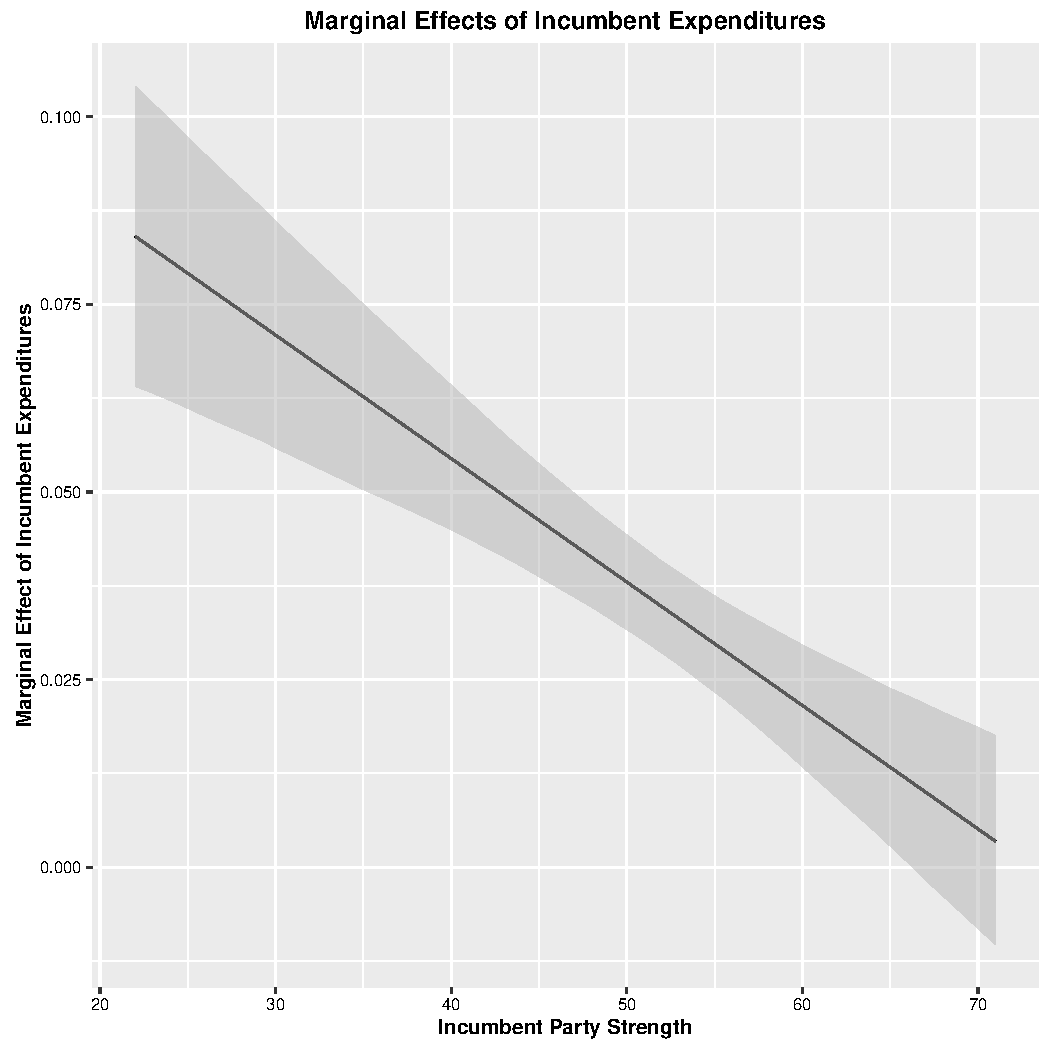
\includegraphics[width=\maxwidth]{figure/unnamed-chunk-3-1} 
\begin{kframe}\begin{alltt}
\hlkwd{library}\hlstd{(interplot)}
\hlkwd{interplot}\hlstd{(}\hlkwc{m} \hlstd{= lm_vote_int,} \hlkwc{var1} \hlstd{=} \hlstr{"prtystrA"}\hlstd{,} \hlkwc{var2} \hlstd{=} \hlstr{"expendA"}\hlstd{)} \hlopt{+} \hlkwd{xlab}\hlstd{(}\hlstr{"Incumbent Expenditures"}\hlstd{)} \hlopt{+}
    \hlkwd{ylab}\hlstd{(}\hlstr{"Marginal Effect of Incumbent Party Strength"}\hlstd{)} \hlopt{+} \hlkwd{ggtitle}\hlstd{(}\hlstr{"Marginal Effects of Incumbent Party Strength"}\hlstd{)} \hlopt{+}
    \hlkwd{theme}\hlstd{(}\hlkwc{plot.title} \hlstd{=} \hlkwd{element_text}\hlstd{(}\hlkwc{face} \hlstd{=} \hlstr{"bold"}\hlstd{,} \hlkwc{size} \hlstd{=} \hlnum{12}\hlstd{),} \hlkwc{axis.title} \hlstd{=} \hlkwd{element_text}\hlstd{(}\hlkwc{size} \hlstd{=} \hlnum{10}\hlstd{,}
        \hlkwc{face} \hlstd{=} \hlstr{"bold"}\hlstd{),} \hlkwc{axis.text} \hlstd{=} \hlkwd{element_text}\hlstd{(}\hlkwc{size} \hlstd{=} \hlnum{8}\hlstd{,} \hlkwc{color} \hlstd{=} \hlstr{"Black"}\hlstd{))}
\end{alltt}
\end{kframe}
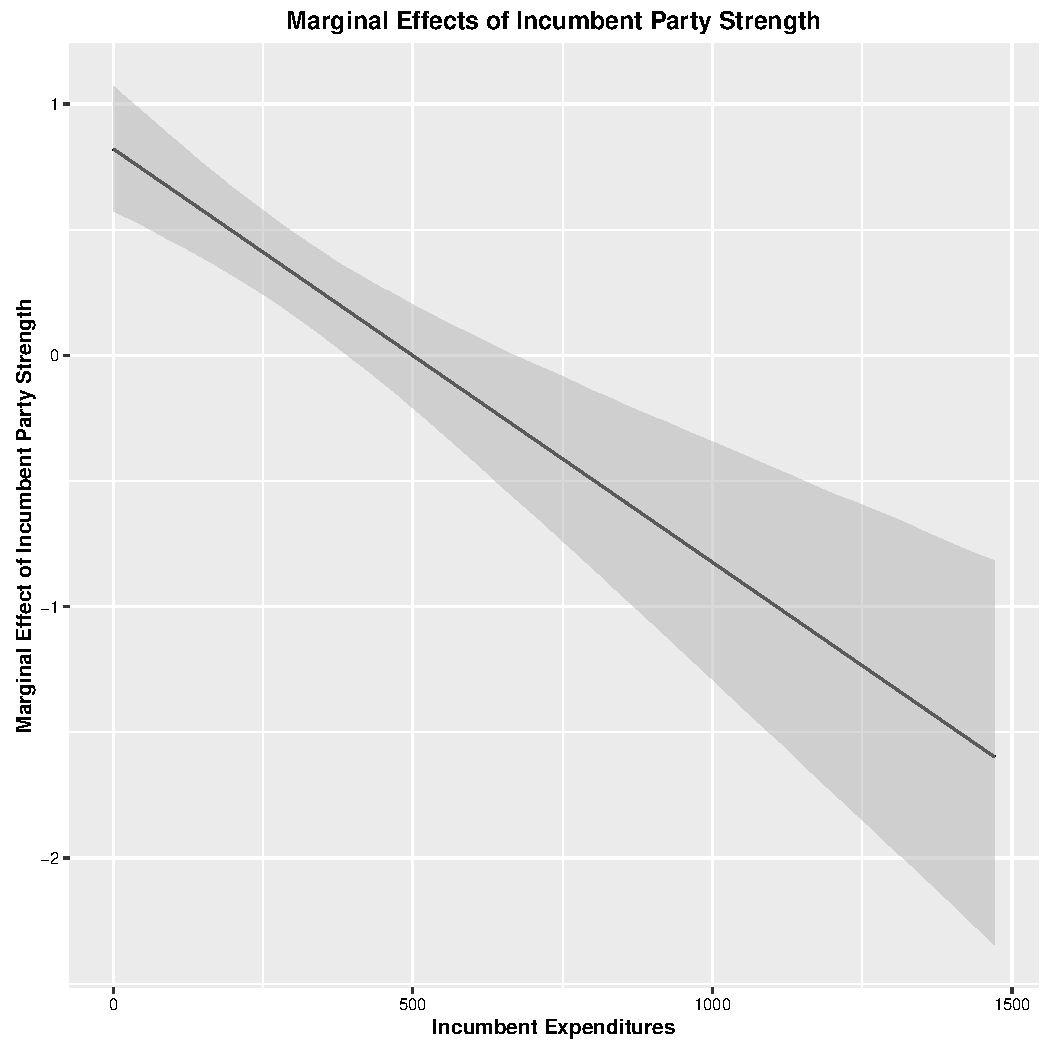
\includegraphics[width=\maxwidth]{figure/unnamed-chunk-3-2} 
\begin{kframe}\begin{alltt}
\hlkwd{library}\hlstd{(coefplot)}
\end{alltt}


{\ttfamily\noindent\itshape\color{messagecolor}{\#\# \\\#\# Attaching package: 'coefplot'}}

{\ttfamily\noindent\itshape\color{messagecolor}{\#\# The following objects are masked from 'package:arm':\\\#\# \\\#\#\ \ \ \  coefplot, coefplot.default}}\begin{alltt}
\hlkwd{buildModelCI}\hlstd{(lm_vote_int)}
\end{alltt}
\begin{verbatim}
##                        Value      Coefficient    HighInner    LowInner
## expendA:prtystrA -0.00164590 expendA:prtystrA -0.001325801 -0.00196600
## prtystrA          0.82330445         prtystrA  0.947669935  0.69893896
## expendB          -0.03391007          expendB -0.031105130 -0.03671501
## expendA           0.12024567          expendA  0.137133916  0.10335743
## (Intercept)       9.07087413      (Intercept) 15.323873796  2.81787446
##                     HighOuter     LowOuter       Model
## expendA:prtystrA -0.001005701 -0.002286099 lm_vote_int
## prtystrA          1.072035425  0.574573465 lm_vote_int
## expendB          -0.028300190 -0.039519951 lm_vote_int
## expendA           0.154022157  0.086469192 lm_vote_int
## (Intercept)      21.576873462 -3.435125201 lm_vote_int
\end{verbatim}
\begin{alltt}
\hlkwd{coefplot}\hlstd{(lm_vote_int,} \hlkwc{coefficients} \hlstd{=} \hlkwd{c}\hlstd{(}\hlstr{"expendA"}\hlstd{,} \hlstr{"prtystrA"}\hlstd{,} \hlstr{"expendA:prtystrA"}\hlstd{),}
    \hlkwc{point} \hlstd{= T)} \hlopt{+} \hlkwd{theme}\hlstd{(}\hlkwc{axis.text.x} \hlstd{=} \hlkwd{element_text}\hlstd{(}\hlkwc{angle} \hlstd{=} \hlnum{90}\hlstd{))}
\end{alltt}
\end{kframe}
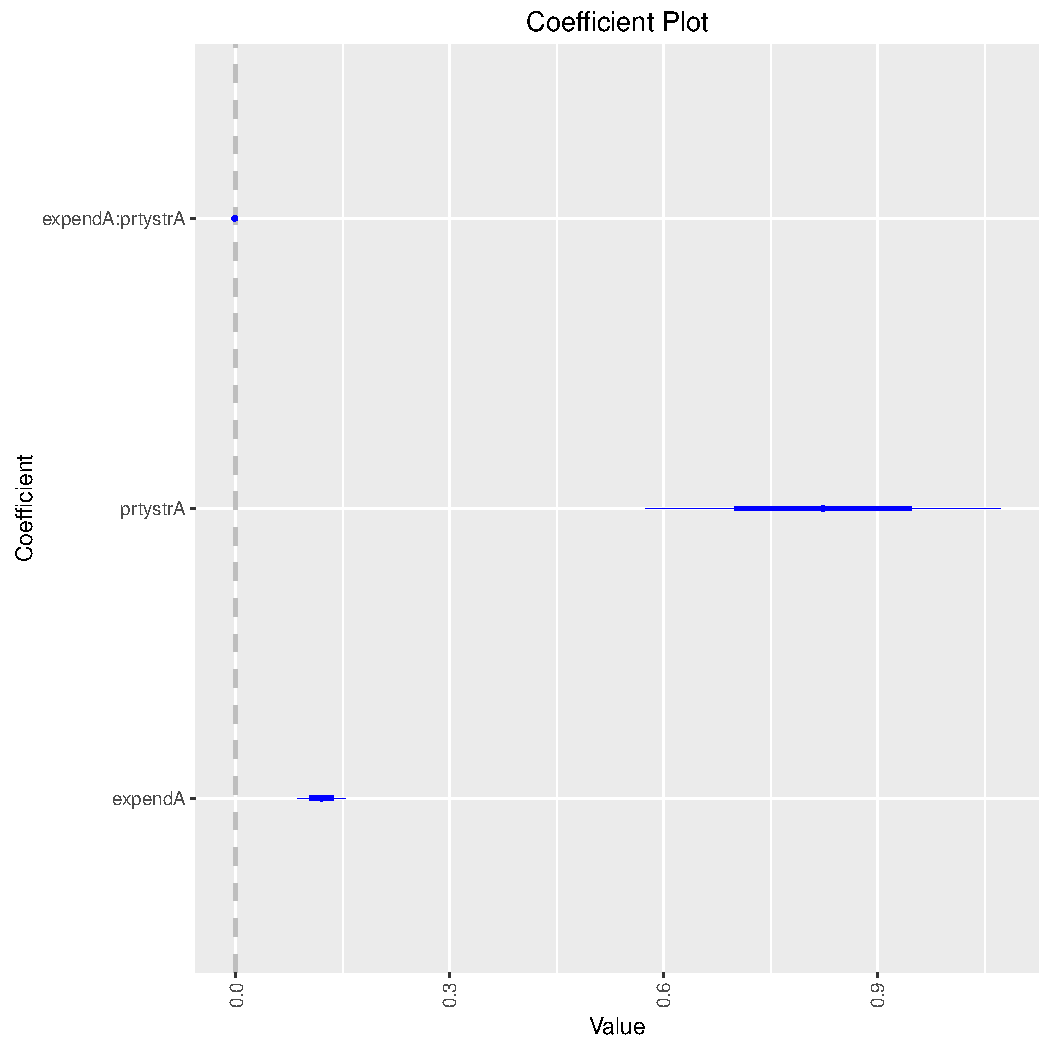
\includegraphics[width=\maxwidth]{figure/unnamed-chunk-3-3} 
\begin{kframe}\begin{alltt}
\hlkwd{coefplot}\hlstd{(lm_vote_int,} \hlkwc{coefficients} \hlstd{=} \hlkwd{c}\hlstd{(}\hlstr{"expendA:prtystrA"}\hlstd{),} \hlkwc{point} \hlstd{= T)} \hlopt{+} \hlkwd{theme}\hlstd{(}\hlkwc{axis.text.x} \hlstd{=} \hlkwd{element_text}\hlstd{(}\hlkwc{angle} \hlstd{=} \hlnum{90}\hlstd{))}
\end{alltt}
\end{kframe}
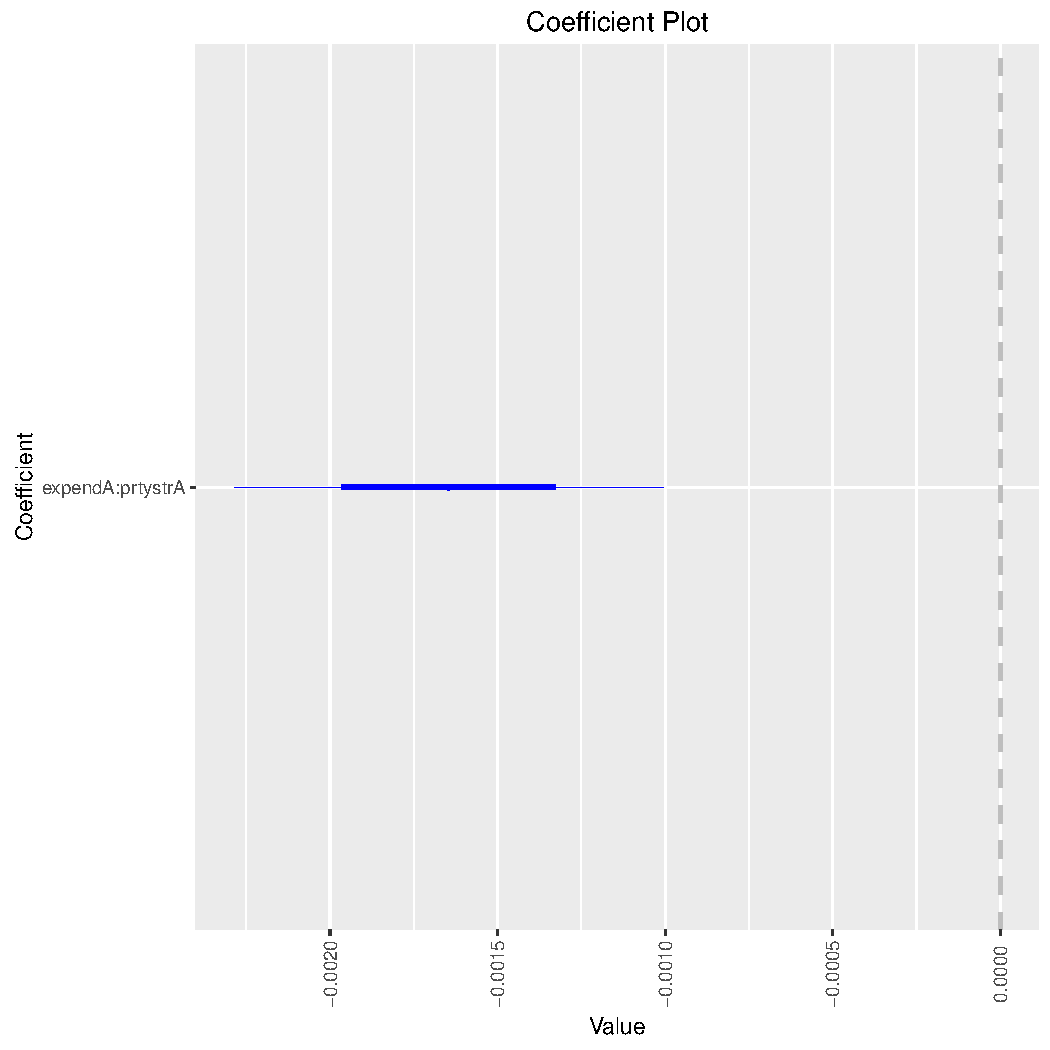
\includegraphics[width=\maxwidth]{figure/unnamed-chunk-3-4} 
\begin{kframe}\begin{alltt}
\hlkwd{quantile}\hlstd{(vote1}\hlopt{$}\hlstd{expendA,} \hlkwc{probs} \hlstd{=} \hlkwd{c}\hlstd{(}\hlnum{0.05}\hlstd{,} \hlnum{0.95}\hlstd{),} \hlkwc{na.rm} \hlstd{=} \hlnum{TRUE}\hlstd{)}
\end{alltt}
\begin{verbatim}
##       5%      95% 
##   8.1354 816.2566
\end{verbatim}
\begin{alltt}
\hlstd{nd1} \hlkwb{=} \hlkwd{data.frame}\hlstd{(}\hlkwc{prtystrA} \hlstd{=} \hlkwd{seq}\hlstd{(}\hlkwd{min}\hlstd{(vote1}\hlopt{$}\hlstd{prtystrA),} \hlkwd{max}\hlstd{(vote1}\hlopt{$}\hlstd{prtystrA),} \hlkwc{length.out} \hlstd{=} \hlnum{10}\hlstd{),}
    \hlkwc{expendA} \hlstd{=} \hlkwd{rep}\hlstd{(}\hlnum{8.1354}\hlstd{,} \hlnum{10}\hlstd{),} \hlkwc{expendB} \hlstd{=} \hlkwd{rep}\hlstd{(}\hlkwd{mean}\hlstd{(vote1}\hlopt{$}\hlstd{expendB),} \hlnum{10}\hlstd{))}
\hlstd{nd2} \hlkwb{=} \hlkwd{data.frame}\hlstd{(}\hlkwc{prtystrA} \hlstd{=} \hlkwd{seq}\hlstd{(}\hlkwd{min}\hlstd{(vote1}\hlopt{$}\hlstd{prtystrA),} \hlkwd{max}\hlstd{(vote1}\hlopt{$}\hlstd{prtystrA),} \hlkwc{length.out} \hlstd{=} \hlnum{10}\hlstd{),}
    \hlkwc{expendA} \hlstd{=} \hlkwd{rep}\hlstd{(}\hlnum{816.2566}\hlstd{,} \hlnum{10}\hlstd{),} \hlkwc{expendB} \hlstd{=} \hlkwd{rep}\hlstd{(}\hlkwd{mean}\hlstd{(vote1}\hlopt{$}\hlstd{expendB),} \hlnum{10}\hlstd{))}

\hlstd{pred.p1} \hlkwb{=} \hlkwd{predict}\hlstd{(lm_vote_int,} \hlkwc{type} \hlstd{=} \hlstr{"response"}\hlstd{,} \hlkwc{se.fit} \hlstd{=} \hlnum{TRUE}\hlstd{,} \hlkwc{newdata} \hlstd{= nd1)}
\hlstd{pred.p2} \hlkwb{=} \hlkwd{predict}\hlstd{(lm_vote_int,} \hlkwc{type} \hlstd{=} \hlstr{"response"}\hlstd{,} \hlkwc{se.fit} \hlstd{=} \hlnum{TRUE}\hlstd{,} \hlkwc{newdata} \hlstd{= nd2)}

\hlstd{pred.table1} \hlkwb{=} \hlkwd{cbind}\hlstd{(pred.p1}\hlopt{$}\hlstd{fit, pred.p1}\hlopt{$}\hlstd{se.fit)}
\hlstd{pred.table2} \hlkwb{=} \hlkwd{cbind}\hlstd{(pred.p2}\hlopt{$}\hlstd{fit, pred.p2}\hlopt{$}\hlstd{se.fit)}

\hlkwd{max}\hlstd{(pred.table1)}
\end{alltt}
\begin{verbatim}
## [1] 57.20747
\end{verbatim}
\begin{alltt}
\hlkwd{max}\hlstd{(pred.table2)}
\end{alltt}
\begin{verbatim}
## [1] 85.43283
\end{verbatim}
\begin{alltt}
\hlkwd{min}\hlstd{(pred.table1)}
\end{alltt}
\begin{verbatim}
## [1] 1.227114
\end{verbatim}
\begin{alltt}
\hlkwd{min}\hlstd{(pred.table2)}
\end{alltt}
\begin{verbatim}
## [1] 1.746126
\end{verbatim}
\begin{alltt}
\hlkwd{plot}\hlstd{(pred.p1}\hlopt{$}\hlstd{fit,} \hlkwc{type} \hlstd{=} \hlstr{"l"}\hlstd{,} \hlkwc{ylim} \hlstd{=} \hlkwd{c}\hlstd{(}\hlnum{0}\hlstd{,} \hlnum{100}\hlstd{),} \hlkwc{main} \hlstd{=} \hlstr{"Predicted Values: Incumbent Vote Share"}\hlstd{,}
    \hlkwc{xlab} \hlstd{=} \hlstr{"Incumbent Party Strength"}\hlstd{,} \hlkwc{ylab} \hlstd{=} \hlstr{"Incumbent Vote Share"}\hlstd{,} \hlkwc{axes} \hlstd{=} \hlnum{FALSE}\hlstd{,}
    \hlkwc{col} \hlstd{=} \hlstr{"blue"}\hlstd{,} \hlkwc{lwd} \hlstd{=} \hlnum{2.5}\hlstd{)}
\hlkwd{axis}\hlstd{(}\hlnum{1}\hlstd{,} \hlkwc{at} \hlstd{=} \hlkwd{seq}\hlstd{(}\hlnum{1}\hlstd{,} \hlnum{10}\hlstd{),} \hlkwc{labels} \hlstd{=} \hlkwd{round}\hlstd{(}\hlkwd{seq}\hlstd{(}\hlkwd{min}\hlstd{(vote1}\hlopt{$}\hlstd{prtystrA),} \hlkwd{max}\hlstd{(vote1}\hlopt{$}\hlstd{prtystrA),}
    \hlkwc{length.out} \hlstd{=} \hlnum{10}\hlstd{),} \hlkwc{digits} \hlstd{=} \hlnum{2}\hlstd{))}
\hlkwd{axis}\hlstd{(}\hlnum{2}\hlstd{,} \hlkwc{at} \hlstd{=} \hlkwd{seq}\hlstd{(}\hlnum{0}\hlstd{,} \hlnum{100}\hlstd{,} \hlkwc{by} \hlstd{=} \hlnum{10}\hlstd{),} \hlkwc{labels} \hlstd{=} \hlkwd{seq}\hlstd{(}\hlnum{0}\hlstd{,} \hlnum{100}\hlstd{,} \hlkwc{by} \hlstd{=} \hlnum{10}\hlstd{))}

\hlcom{# Add lines}

\hlkwd{lines}\hlstd{(pred.p1}\hlopt{$}\hlstd{fit,} \hlkwc{col} \hlstd{=} \hlstr{"blue"}\hlstd{,} \hlkwc{lwd} \hlstd{=} \hlnum{2.5}\hlstd{)}
\hlkwd{lines}\hlstd{(pred.p2}\hlopt{$}\hlstd{fit,} \hlkwc{col} \hlstd{=} \hlstr{"red"}\hlstd{,} \hlkwc{lwd} \hlstd{=} \hlnum{2.5}\hlstd{)}

\hlcom{# Add legend}

\hlkwd{legend}\hlstd{(}\hlstr{"bottomright"}\hlstd{,} \hlkwd{c}\hlstd{(}\hlstr{"Low Incumbent Expenditures"}\hlstd{,} \hlstr{"High Incumbent Expenditures"}\hlstd{),}
    \hlkwc{lty} \hlstd{=} \hlnum{1}\hlstd{,} \hlkwc{lwd} \hlstd{=} \hlnum{2}\hlstd{,} \hlkwc{col} \hlstd{=} \hlkwd{c}\hlstd{(}\hlstr{"blue"}\hlstd{,} \hlstr{"red"}\hlstd{),} \hlkwc{bty} \hlstd{=} \hlstr{"n"}\hlstd{,} \hlkwc{cex} \hlstd{=} \hlnum{1.25}\hlstd{)}

\hlcom{# Add confidence intervals}

\hlstd{fit1} \hlkwb{=} \hlstd{pred.p1}\hlopt{$}\hlstd{fit}
\hlstd{low1} \hlkwb{=} \hlstd{pred.p1}\hlopt{$}\hlstd{fit} \hlopt{-} \hlnum{2} \hlopt{*} \hlstd{pred.p1}\hlopt{$}\hlstd{se.fit}
\hlstd{high1} \hlkwb{=} \hlstd{pred.p1}\hlopt{$}\hlstd{fit} \hlopt{+} \hlnum{2} \hlopt{*} \hlstd{pred.p1}\hlopt{$}\hlstd{se.fit}
\hlstd{cis1} \hlkwb{=} \hlkwd{cbind}\hlstd{(fit1, low1, high1)}

\hlstd{fit2} \hlkwb{=} \hlstd{pred.p2}\hlopt{$}\hlstd{fit}
\hlstd{low2} \hlkwb{=} \hlstd{pred.p2}\hlopt{$}\hlstd{fit} \hlopt{-} \hlnum{2} \hlopt{*} \hlstd{pred.p2}\hlopt{$}\hlstd{se.fit}
\hlstd{high2} \hlkwb{=} \hlstd{pred.p2}\hlopt{$}\hlstd{fit} \hlopt{+} \hlnum{2} \hlopt{*} \hlstd{pred.p2}\hlopt{$}\hlstd{se.fit}
\hlstd{cis2} \hlkwb{=} \hlkwd{cbind}\hlstd{(fit2, low2, high2)}

\hlkwd{matlines}\hlstd{(cis1[,} \hlkwd{c}\hlstd{(}\hlnum{2}\hlstd{,} \hlnum{3}\hlstd{)],} \hlkwc{lty} \hlstd{=} \hlnum{2}\hlstd{,} \hlkwc{col} \hlstd{=} \hlstr{"blue"}\hlstd{)}
\hlkwd{matlines}\hlstd{(cis2[,} \hlkwd{c}\hlstd{(}\hlnum{2}\hlstd{,} \hlnum{3}\hlstd{)],} \hlkwc{lty} \hlstd{=} \hlnum{2}\hlstd{,} \hlkwc{col} \hlstd{=} \hlstr{"red"}\hlstd{)}
\end{alltt}
\end{kframe}
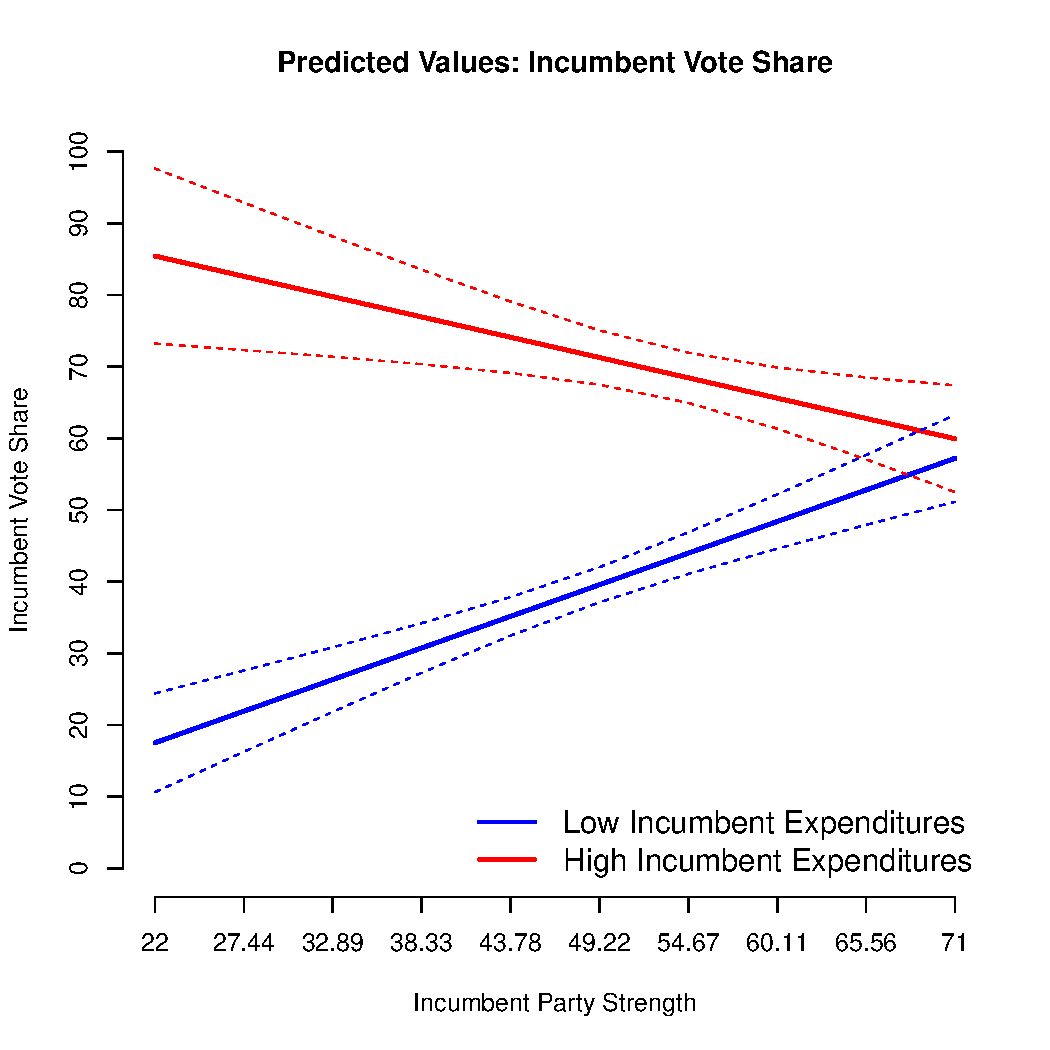
\includegraphics[width=\maxwidth]{figure/unnamed-chunk-3-5} 

\end{knitrout}

\paragraph{d)}

\begin{enumerate}
  \item A lower level of incumbent party strength is associated with a more positive effect of incumbent party expenditures. This is so because, due to the negative coefficient of the interaction term, for decreases in incumbent party strength, we will see an increase in the marginal effect of incumbent party expenditures.
  \item A higher level of incumbent party expenditures is associated with a more negative effect of incumbent party strength. This is so because, due to the negative coefficient of the interaction term, for increases in incumbent party expenditures, we will see a decrease in the marginal effect of incumbent party strength.
\end{enumerate}



\section*{Interactions: Math and Interpretation}

\subsection*{Problem 3}

\paragraph*{a)}

\begin{displaymath}

\dfrac{\partial Y}{\partial X_1} = 5 + X_2

\bigskip

\dfrac{\partial Y}{\partial X_2} = 2 + X_1

\end{displaymath}

\paragraph*{b)}

\begin{knitrout}
\definecolor{shadecolor}{rgb}{0.969, 0.969, 0.969}\color{fgcolor}\begin{kframe}
\begin{alltt}
\hlstd{x2} \hlkwb{=} \hlkwd{seq}\hlstd{(}\hlopt{-}\hlnum{10}\hlstd{,} \hlnum{10}\hlstd{)}

\hlstd{marginal_effect_x1} \hlkwb{=} \hlkwd{rep}\hlstd{(}\hlnum{5}\hlstd{,} \hlnum{21}\hlstd{)} \hlopt{+} \hlstd{x2}

\hlkwd{plot}\hlstd{(x2, marginal_effect_x1,} \hlkwc{main} \hlstd{=} \hlstr{"Marginal Effect of X1"}\hlstd{,} \hlkwc{xlab} \hlstd{=} \hlstr{"X2"}\hlstd{,} \hlkwc{ylab} \hlstd{=} \hlstr{"Marginal Effect of X1"}\hlstd{)}
\end{alltt}
\end{kframe}
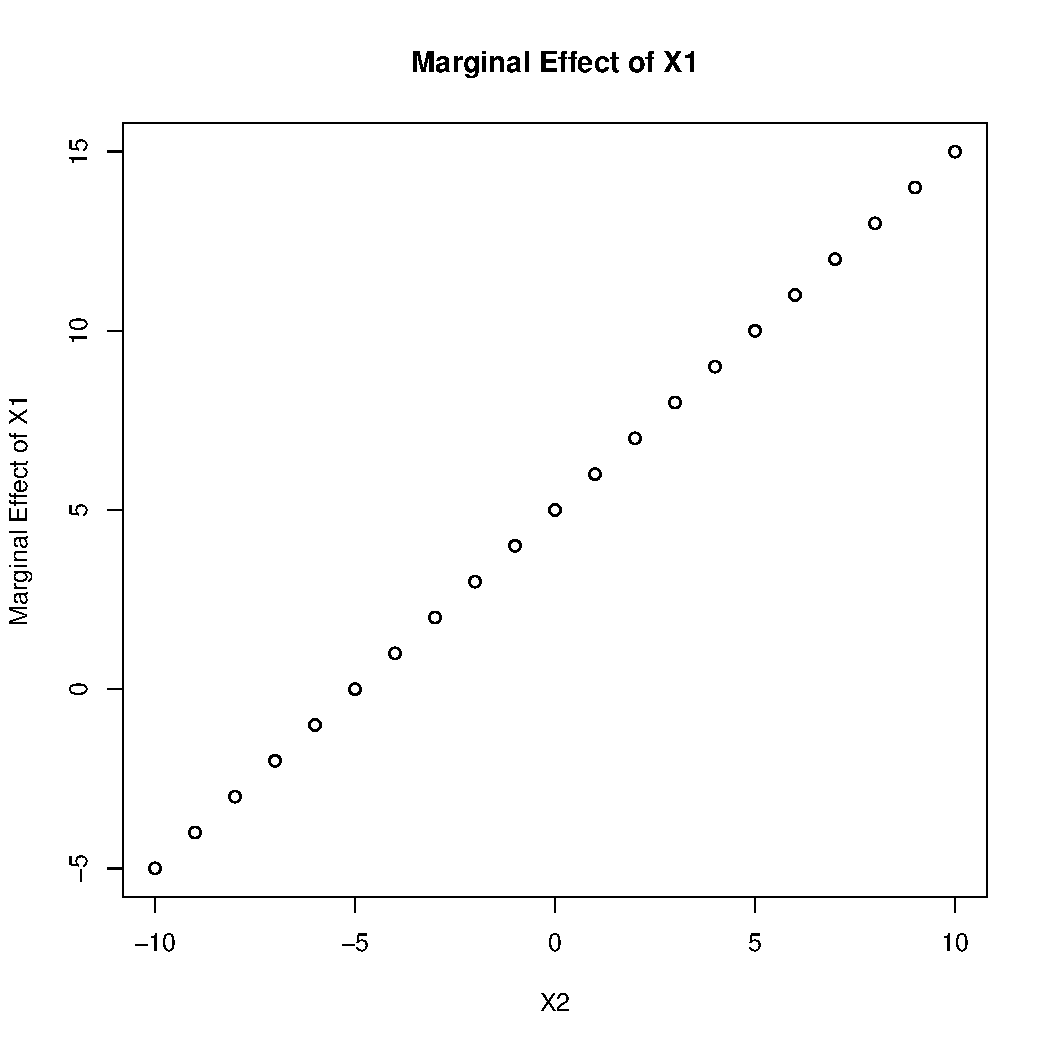
\includegraphics[width=\maxwidth]{figure/unnamed-chunk-4-1} 

\end{knitrout}

\paragraph*{c)} When $X_2$ is at a value of 0, for a 1-unit increase in $X_1$, we would expect a 5 unit increase in Y.

Generally, for a 1-unit increase in $X_1$, we would expect a $5 + X_2$ increase in Y.

\paragraph*{d)}

If an interaction exists in reality and we omit the interaction term from our model, we will introduce a bias to our coefficients. The reason for this is that situations in which a high value in Y is caused by jointly high values in $X_1$ and $X_2$ will not be correctly captured by the model. Instead, high values in Y will incorrectly be attributed to either $X_1$ or $X_2$, but not to their interaction.

\end{document}
